\section{Planning and Implementation}
\label{sec:implementation}

\subsection{Initial Setup and OS install}
\label{subsec:initial-install}
\subsubsection{Install - balenaEtcher}
\label{subsubsec:balena-install}
To start the install I used balenaEtcher \parencite{Balena2024Etcher} with a downloaded .iso disk image of Ubuntu server (24.04 LTS), figures \ref{fig:balena1}, \ref{fig:balena2} and \ref{fig:balena3} show the install process though balenaEtcher's ui to configure the OS, select the medium (again the coursework provided SD card) and begin the installation. However, figure \ref{fig:balena4} shows the bootloader after installing the OS and installing the SD card into the Pi, suggesting the install didn't go well.

\begin{figure}[H]
\centering
\begin{minipage}{.48\textwidth}
  \centering
  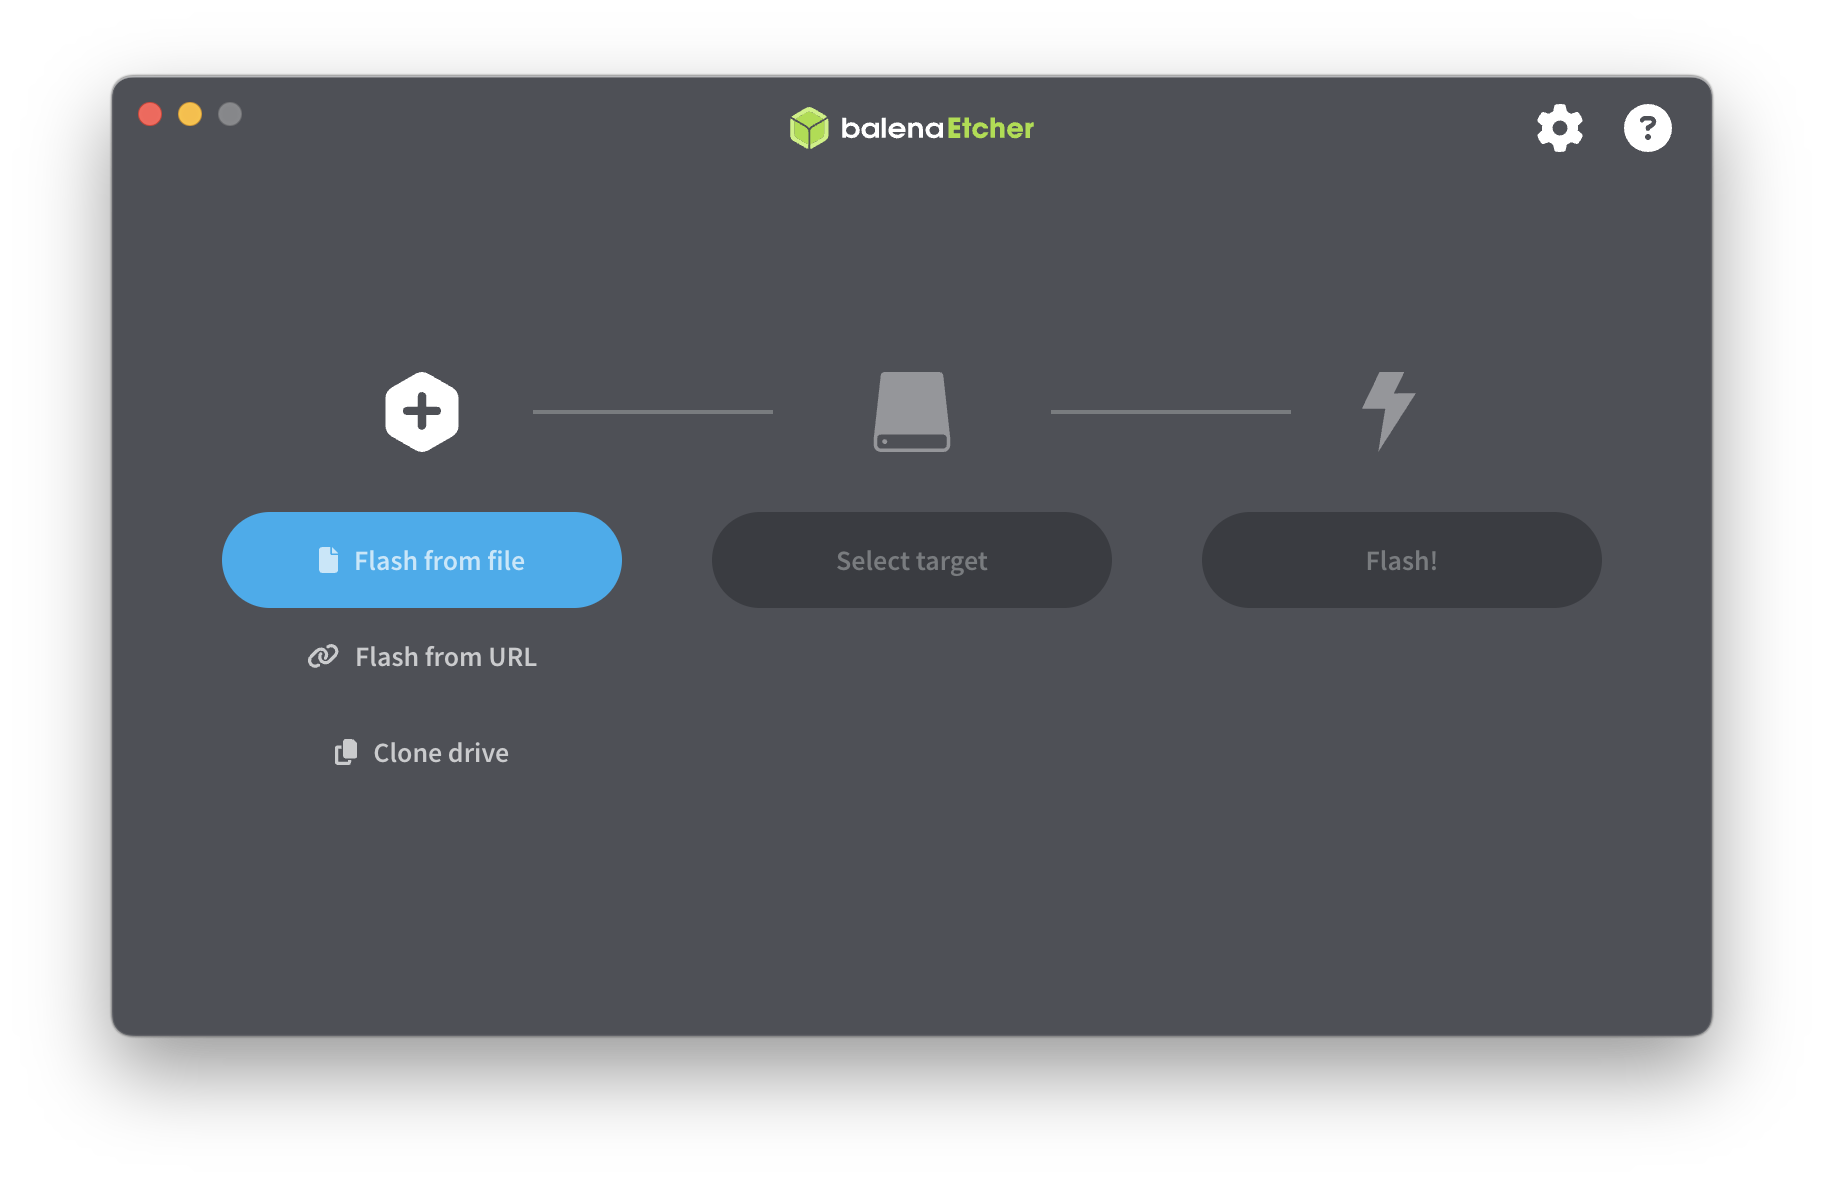
\includegraphics[width=.9\linewidth]{Install_Images/os-balenaetcher-install.png}
  \captionof{figure}{Balena Etcher interface ready to flash the Ubuntu Server image to the SD card.}
  \label{fig:balena1}
\end{minipage}\hfill
\begin{minipage}{.48\textwidth}
  \centering
  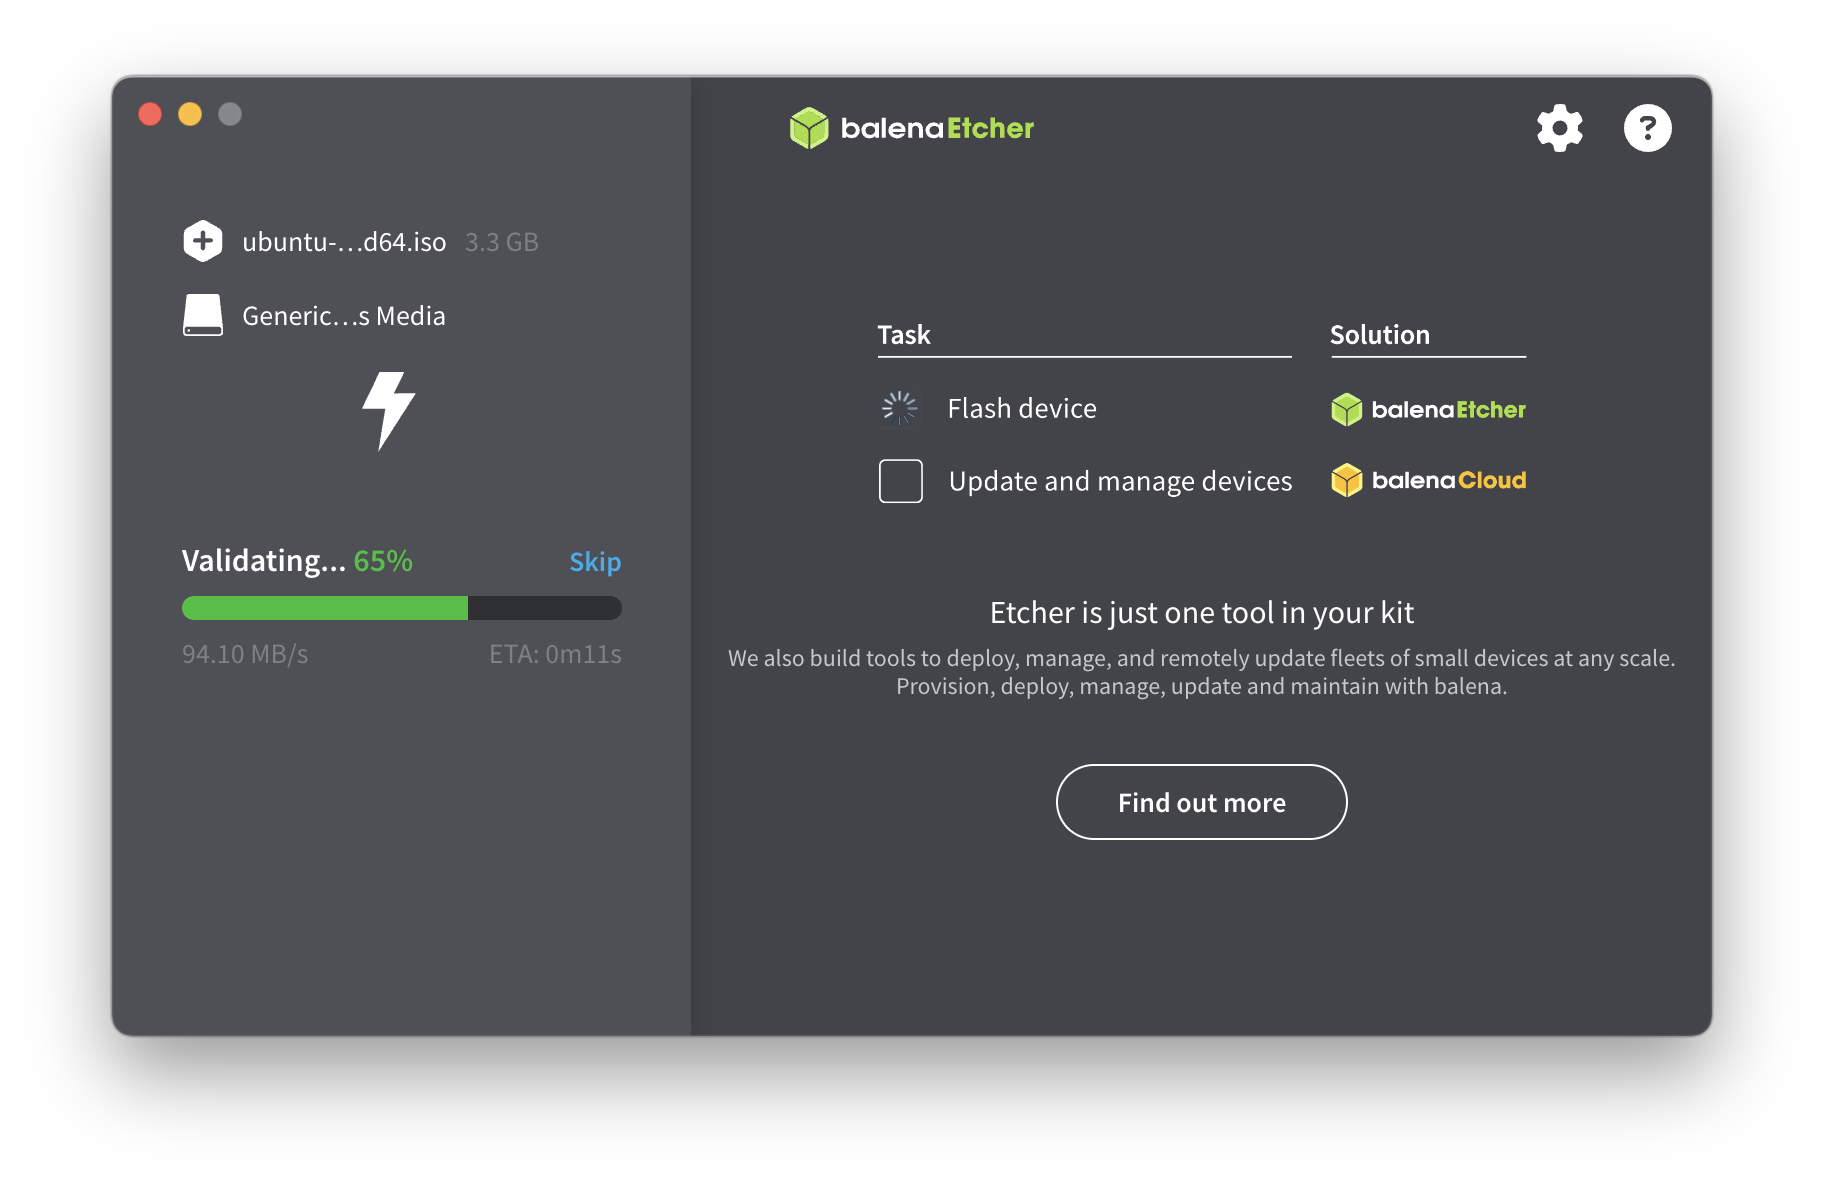
\includegraphics[width=.9\linewidth]{Install_Images/os-balenaetcher-validate.png}
  \captionof{figure}{Balena Etcher validating the written image to ensure data integrity.}
  \label{fig:balena2}
\end{minipage}
\end{figure}

\begin{figure}[H]
\centering
\begin{minipage}{.48\textwidth}
  \centering
  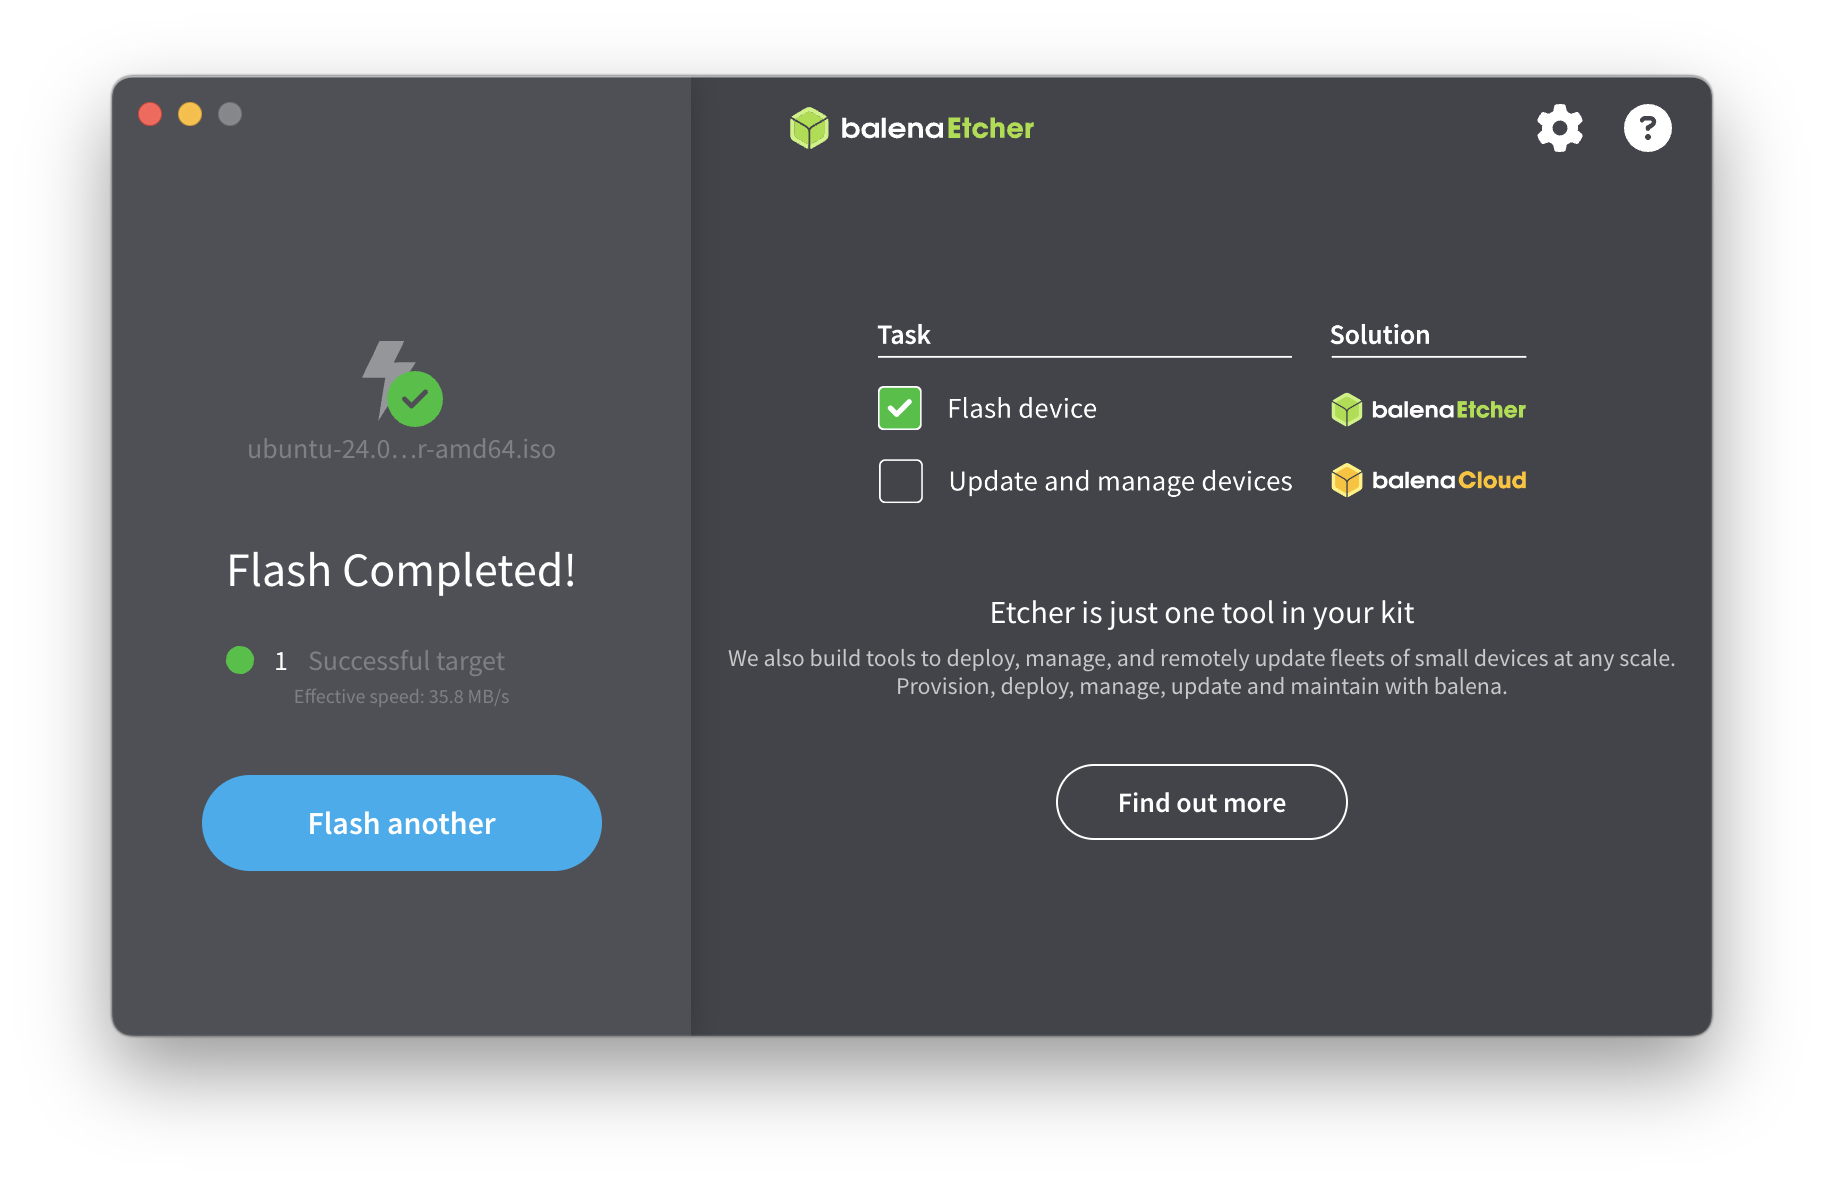
\includegraphics[width=.9\linewidth]{Install_Images/os-balenaetcher-finished.png}
  \captionof{figure}{Balena Etcher reporting successful completion of the flash operation.}
  \label{fig:balena3}
\end{minipage}\hfill
\begin{minipage}{.48\textwidth}
  \centering
  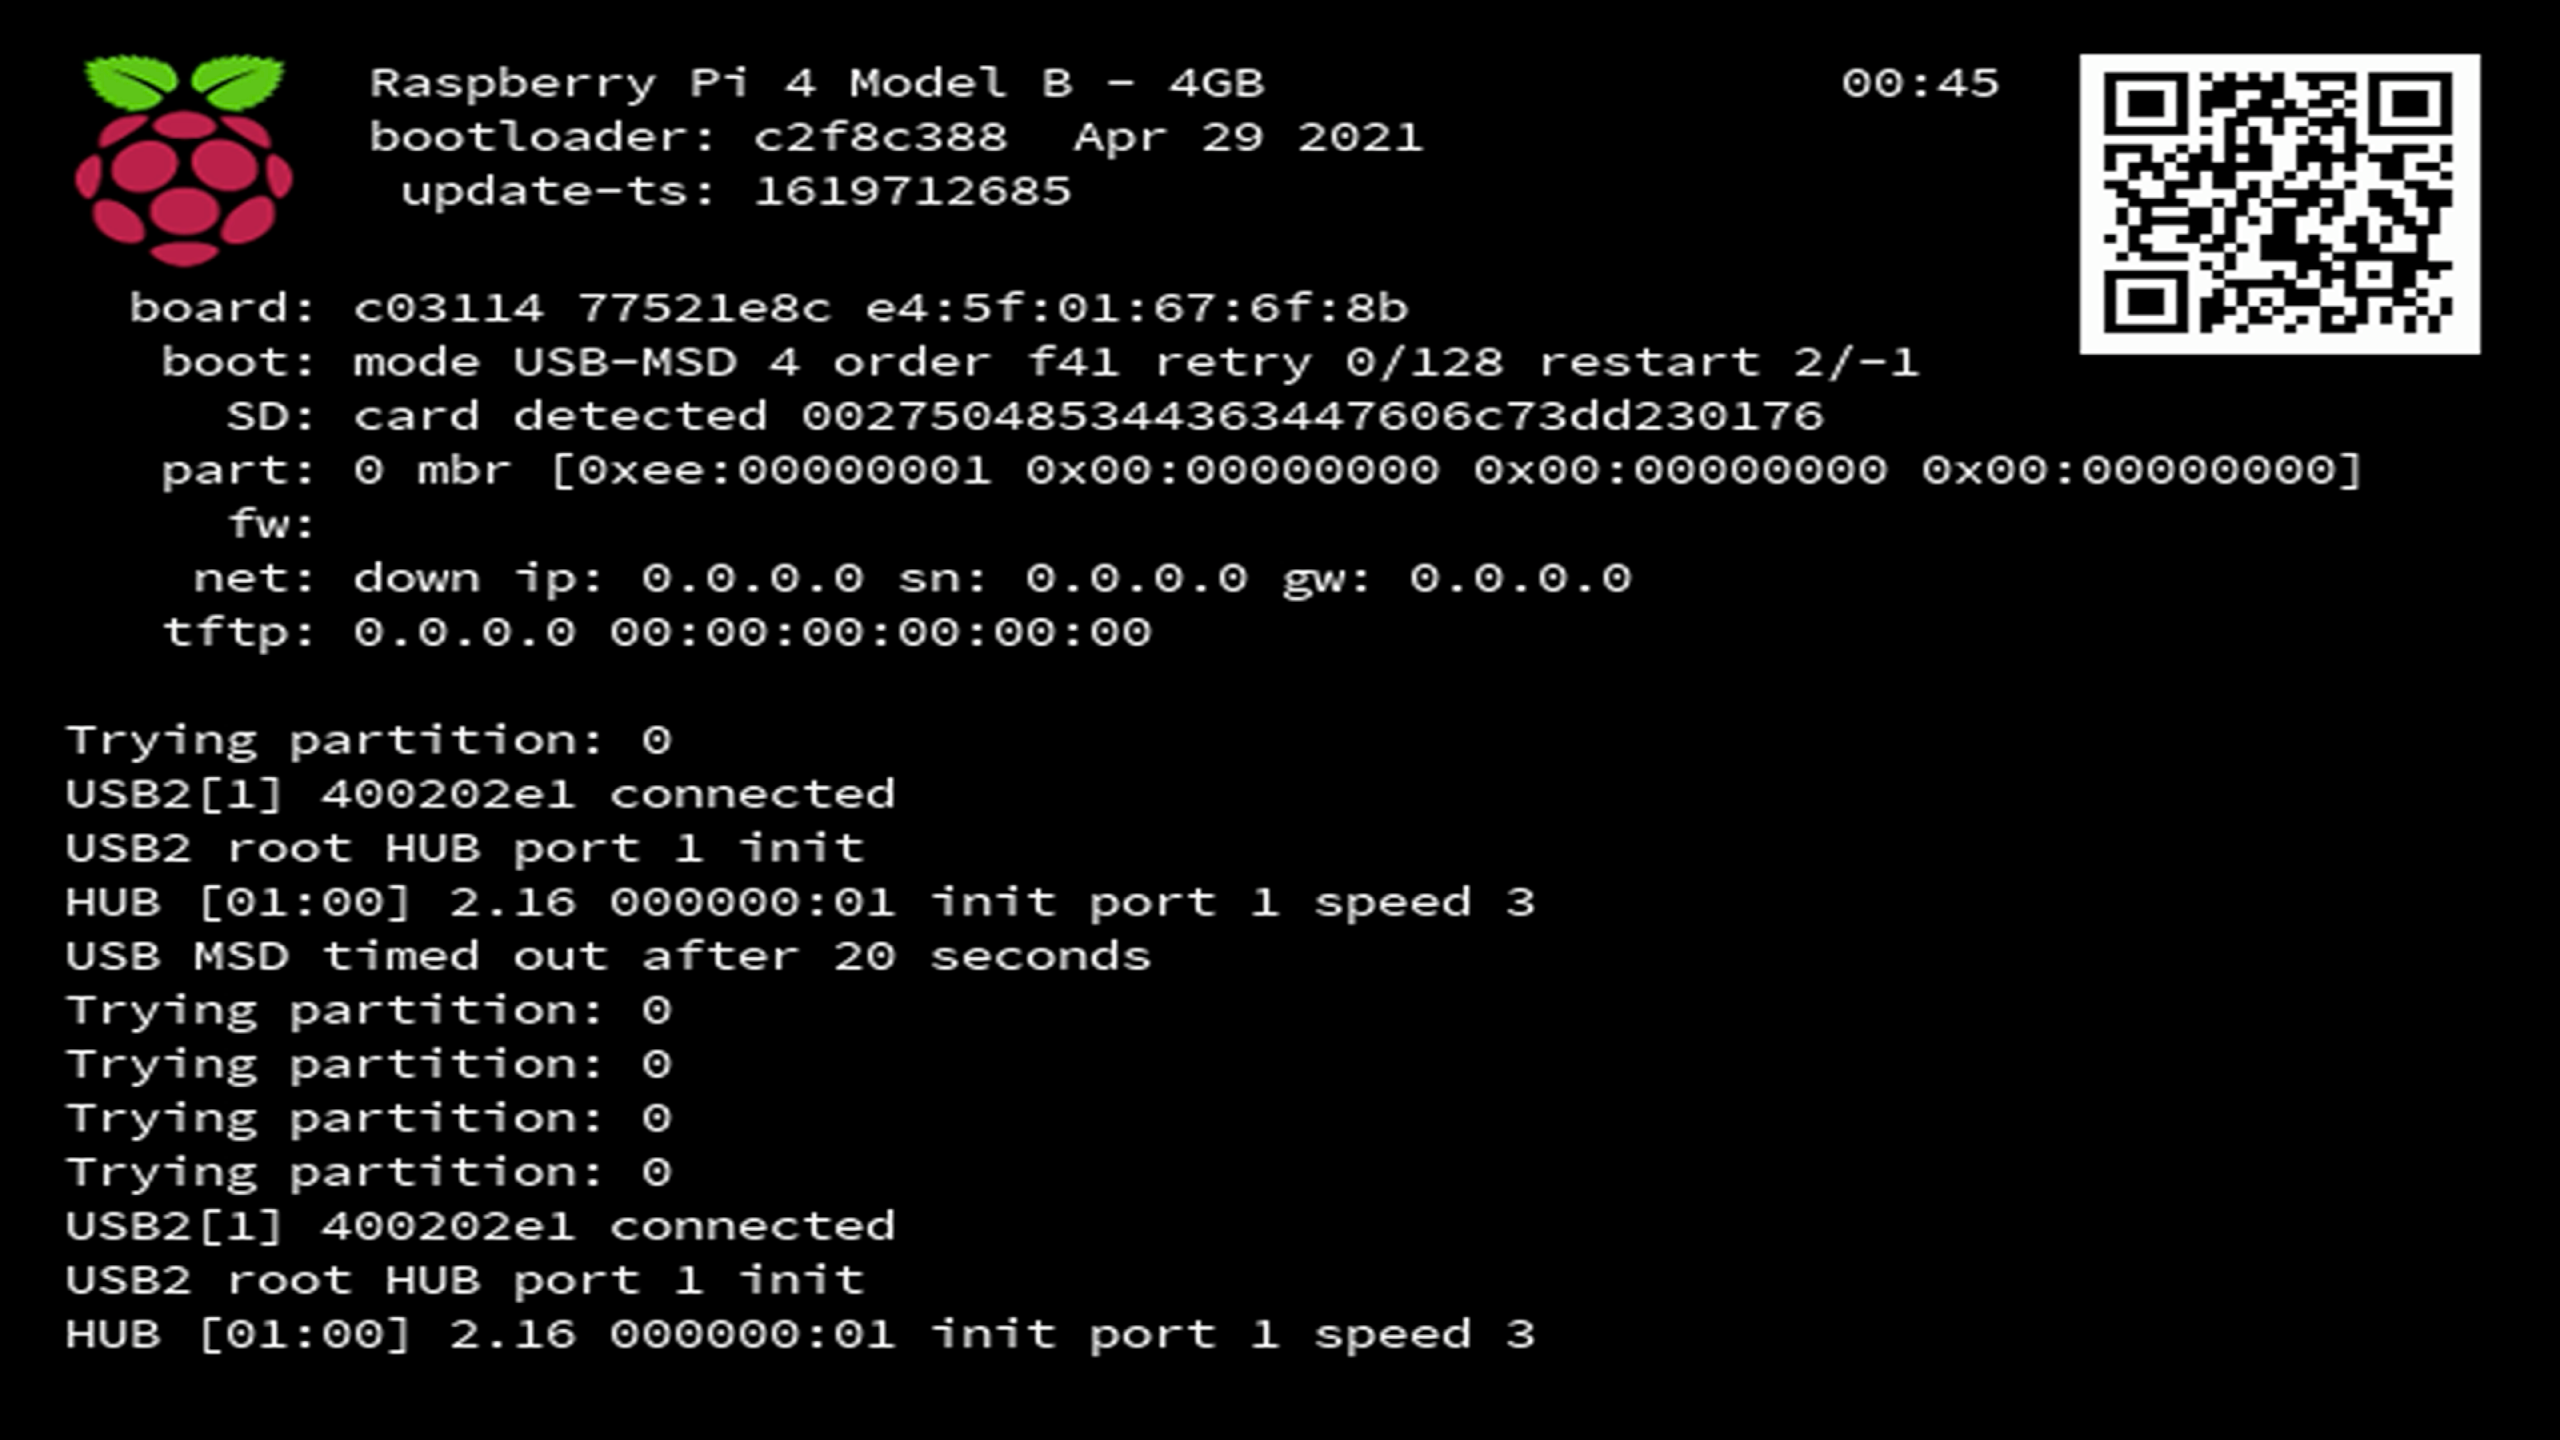
\includegraphics[width=.9\linewidth]{Install_Images/os-balenaetcher-fail-bootloader.png}
  \captionof{figure}{Raspberry Pi 4 bootloader failure}
  \label{fig:balena4}
\end{minipage}
\end{figure}

However, when I installed the SD card into the Raspberry Pi and powered it on, the system failed to boot successfully. Figure \ref{fig:balena4} shows the bootloader, not something you want to see. The error messages show:
\begin{itemize}
    \item \texttt{USB MSD timed out after 20 seconds} - The bootloader tried to read from the SD card but went past the timeout threshold
    \item \texttt{Trying partition: 0} - The bootloader detected no valid bootable partitions on the SD card
\end{itemize}

The boot failure highlights the firmware compatibility between the operating system image and the device's bootloader. Unlike traditional x86 BIOS/UEFI-based computers that follow a standardised boot spec, ARM-based SBCs sometimes need vendor-specific boot configurations like the Raspberry Pi Imager \parencite{RaspberryPi2024Imager}.

\subsubsection{Install - Raspberry Pi Imager}
\label{subsubsec:balena-install}
Following the balenaEtcher failure, I reattempted the install using the Raspberry Pi Imager \parencite{RaspberryPi2024Imager}. Unlike balenaEtcher (a generic disk imager), the Raspberry Pi Imager is purpose-built for Raspberry Pi hardware and automatically applies board-specific boot configurations, firmware updates, and more importantly, first-boot customisation options, so you can run the Pi over a local network (configuring an SSH server, credentials and providing hard-coded network information). Figure \ref{fig:install-base} shows the Raspberry Pi Imager interface with the device model (Raspberry Pi 4), operating system (Ubuntu Server 24.04 LTS 64-bit), and storage medium (SD card) selected.

\begin{figure}[H]
    \centering
    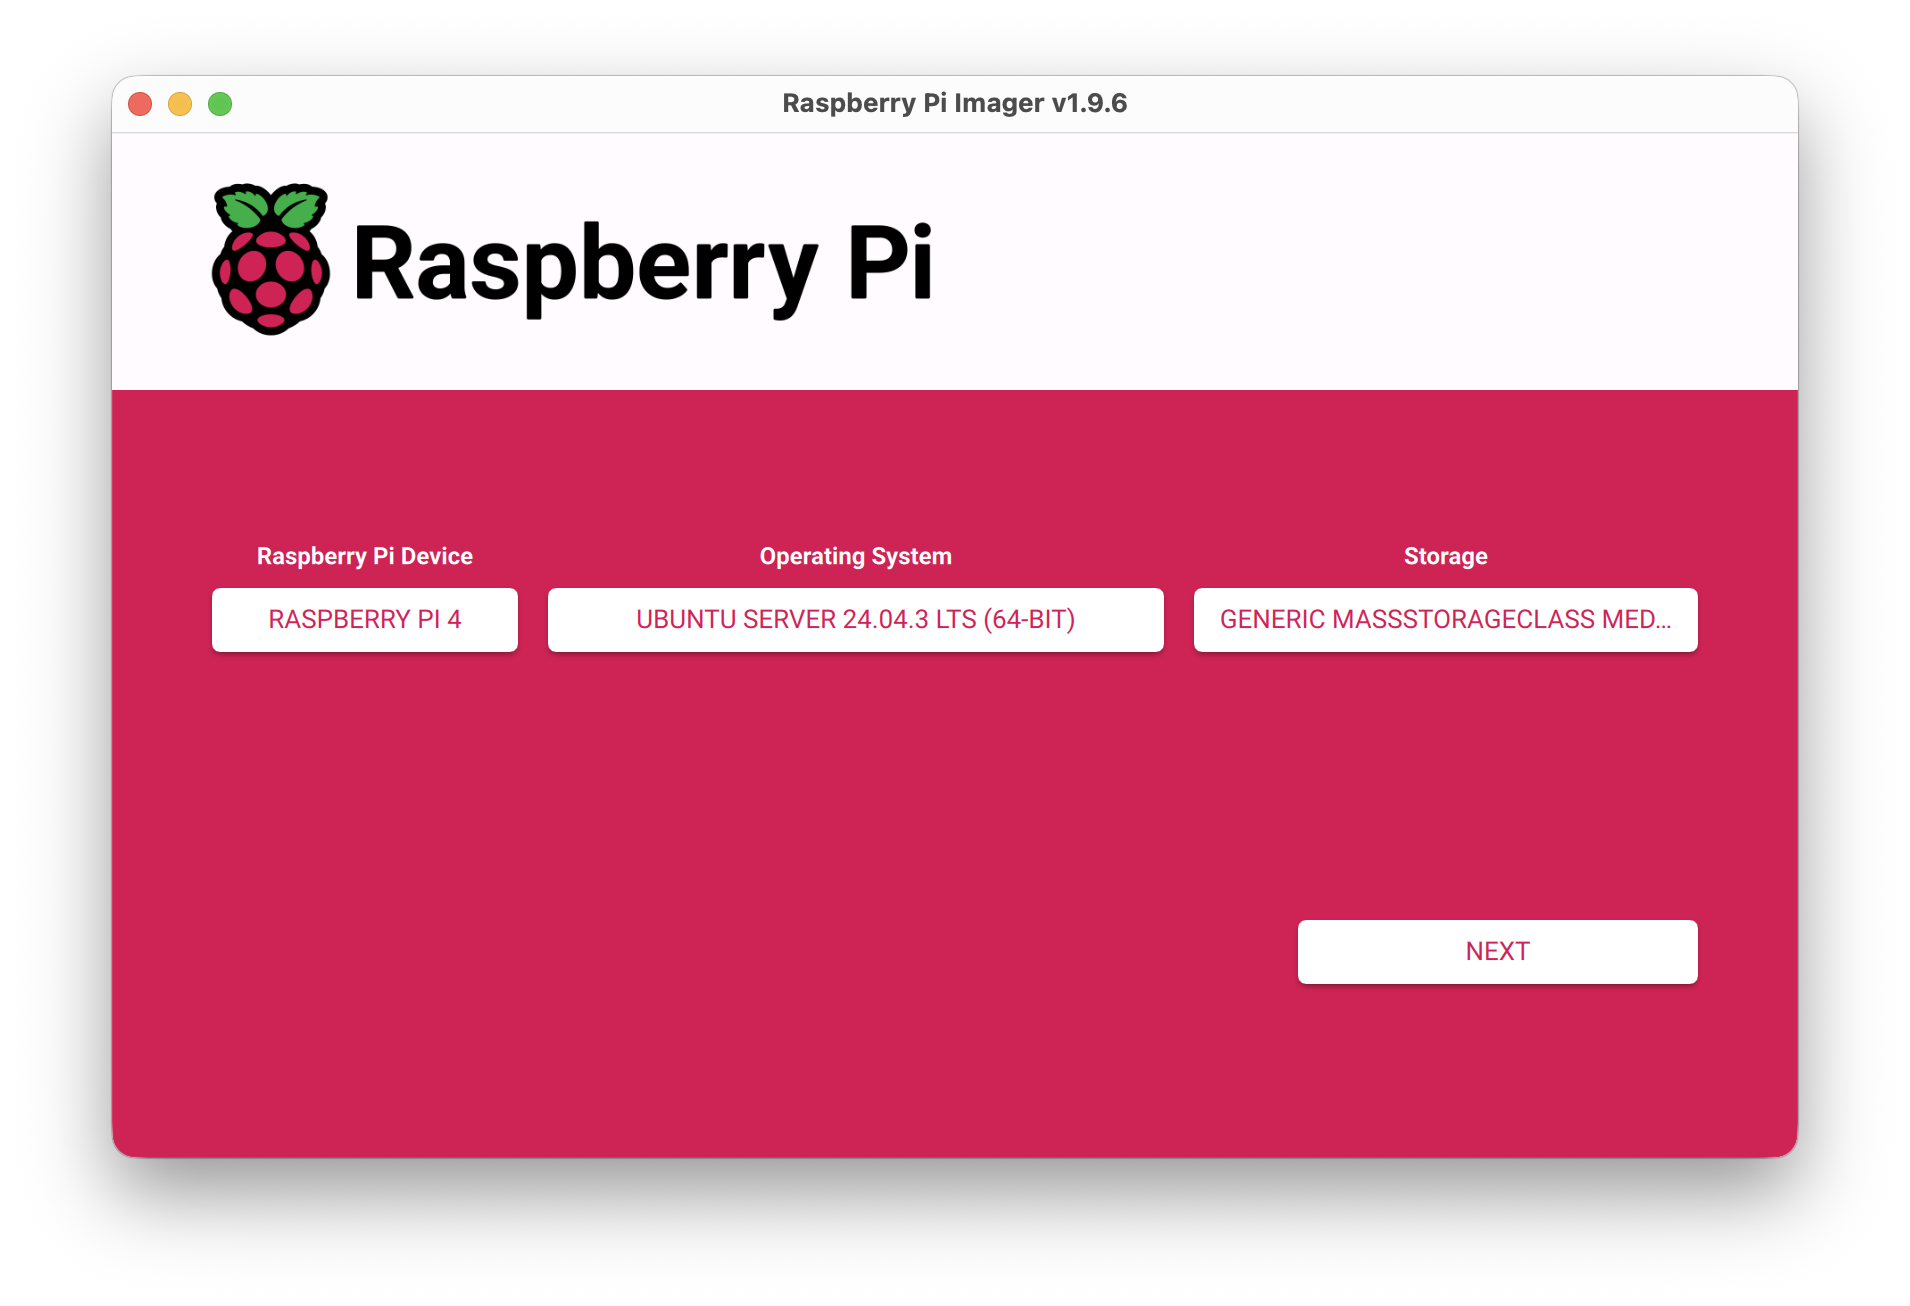
\includegraphics[width=0.7\linewidth]{Install_Images/os-raspi-imager-setup.png}
    \caption{Raspberry Pi Imager main interface showing device, OS, and storage selection before customization.}
    \label{fig:raspi-setup}
\end{figure}

Before writing the image, the Imager prompted for OS customization settings (Figure \ref{fig:raspi-extra-select}), which enables headless deployment without requiring physical access to the Raspberry Pi for initial configuration.

\begin{figure}[H]
\centering
\begin{minipage}{.48\textwidth}
  \centering
  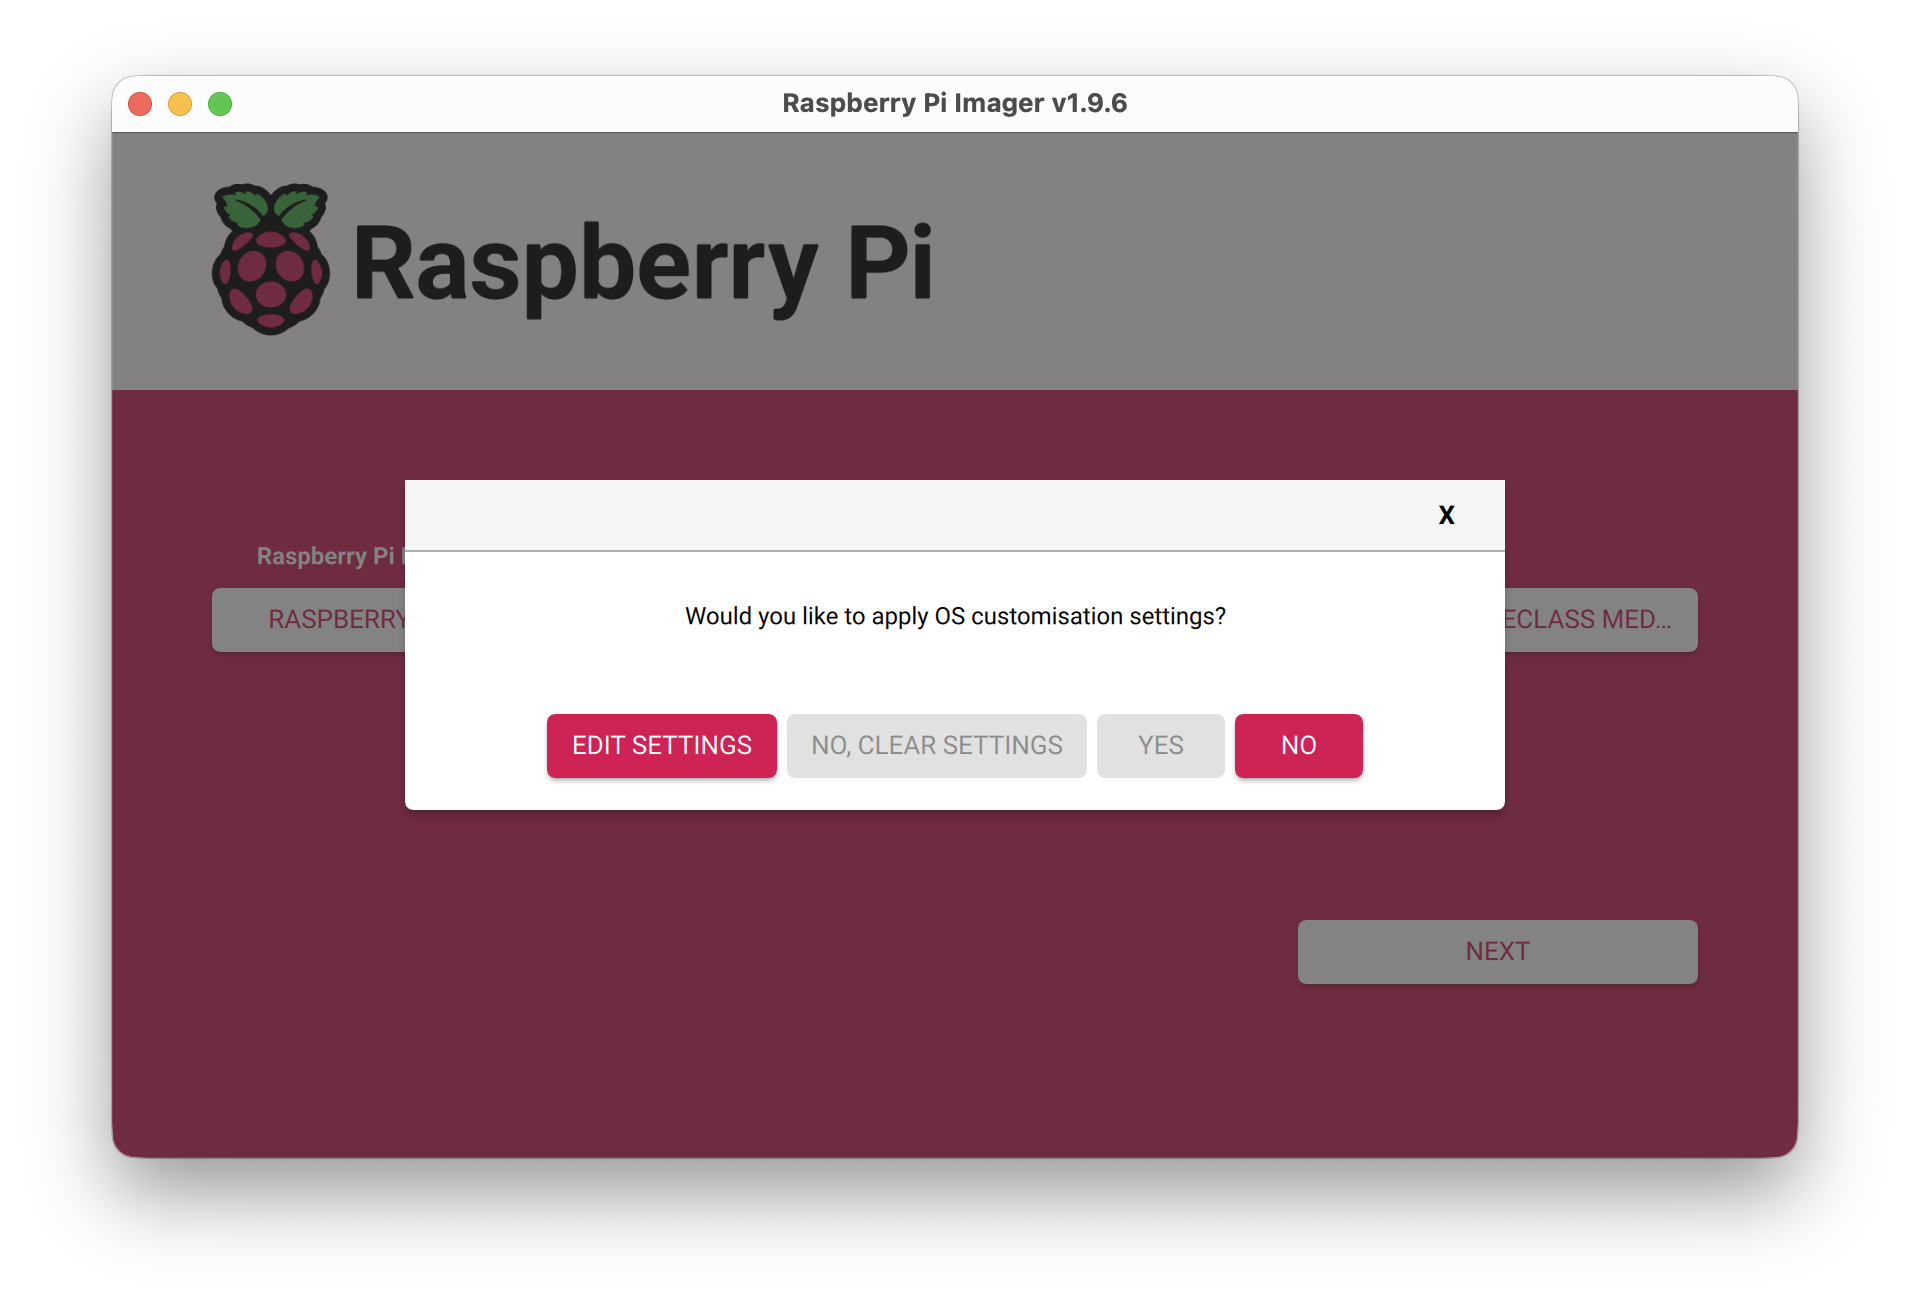
\includegraphics[width=.9\linewidth]{Install_Images/os-raspi-imager-extra-select.png}
  \captionof{figure}{OS customization prompt offering pre-boot configuration options.}
  \label{fig:raspi-extra-select}
\end{minipage}\hfill
\begin{minipage}{.48\textwidth}
  \centering
  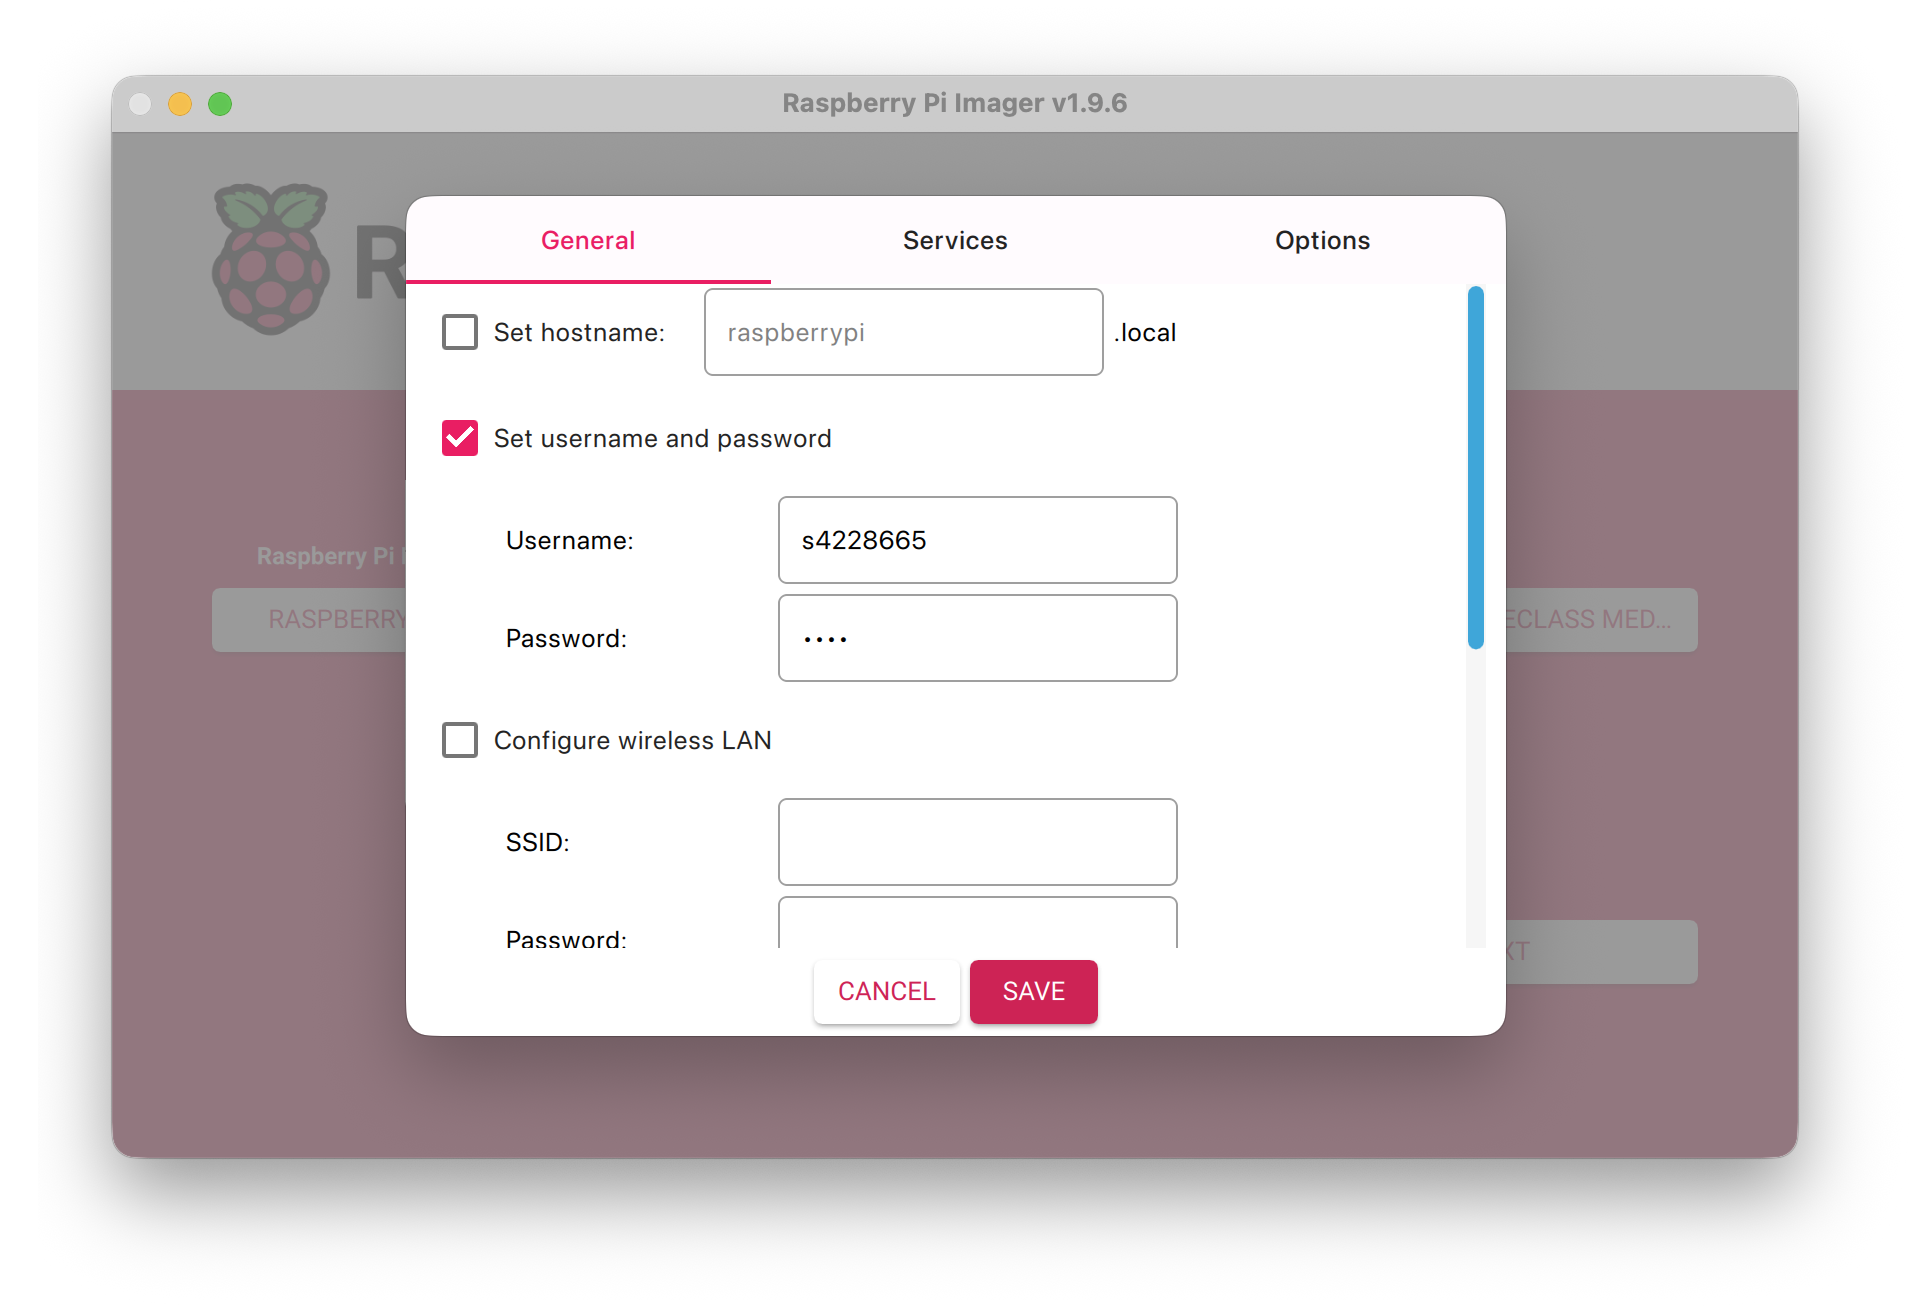
\includegraphics[width=.9\linewidth]{Install_Images/os-raspi-imager-extra.png}
  \captionof{figure}{Customization dialog showing my username (s4228665)}
  \label{fig:raspi-extra}
\end{minipage}
\end{figure}

The OS customisation fields (Figure \ref{fig:raspi-extra}) show I configured:
\begin{itemize}
    \item \textbf{Username}: \texttt{s4228665} (my student ID)
    \item \textbf{Hostname}: \texttt{raspberrypi.local} - left as default so it can be provisioned by Ansible (section \ref{sec:provision.yml})
    \item \textbf{Wireless LAN}: SSID and password - also left as default so it can be provisioned by Ansible (section \ref{sec:netplan.yml})
\end{itemize}

After confirming settings, the Imager wrote the image to the SD card (Figure \ref{fig:raspi-writing}).

\begin{figure}[H]
    \centering
    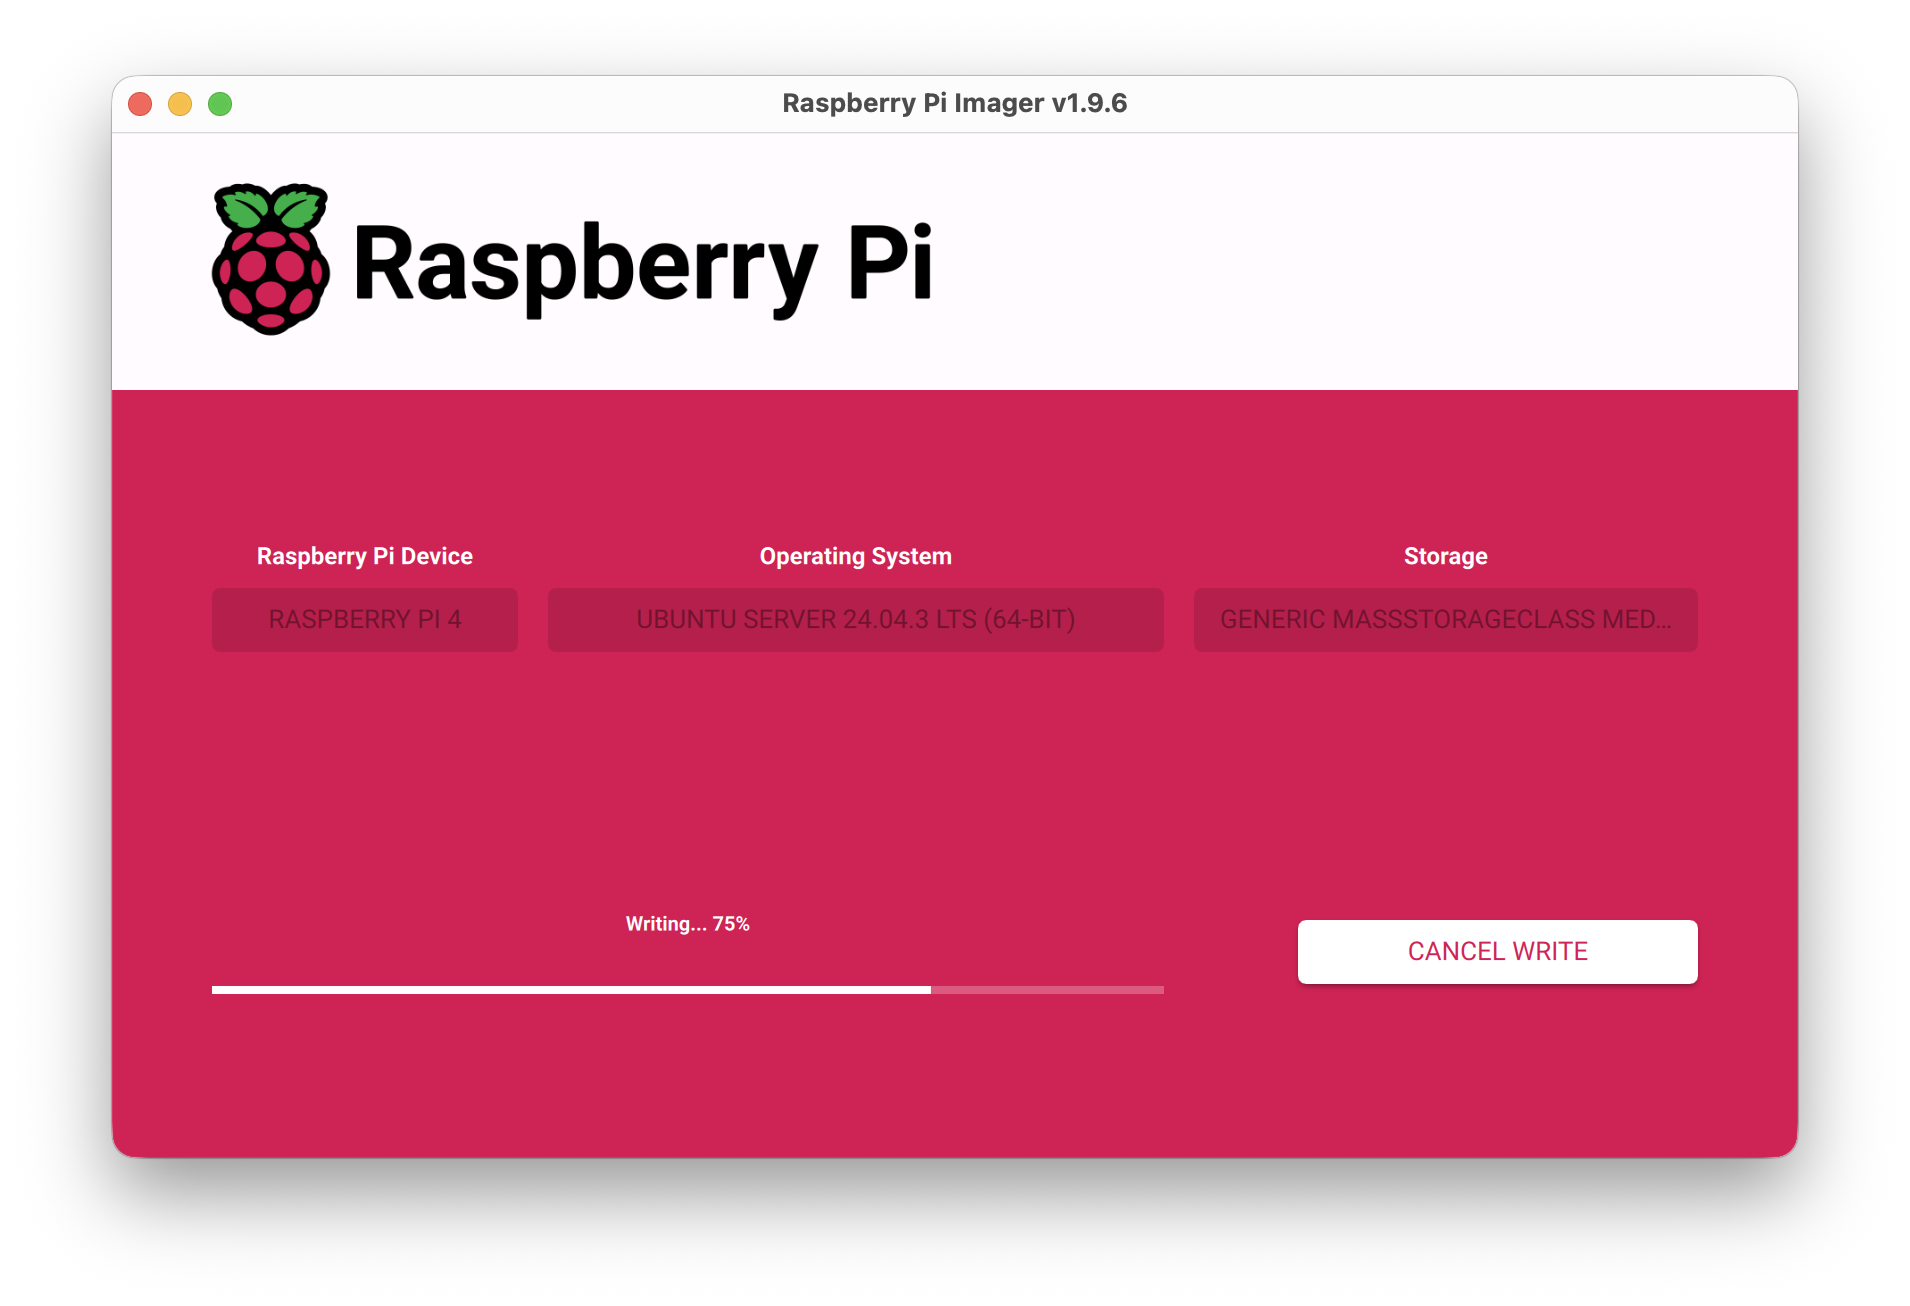
\includegraphics[width=0.7\linewidth]{Install_Images/os-raspi-imager-writing.png}
    \caption{The Imager at 75\% progress}
    \label{fig:raspi-writing}
\end{figure}

\subsubsection{First Boot and Initial Configuration}
\label{subsubsec:first-boot}

After inserting the SD card and turning on the Pi, the system booted into the OS, then started generating SSH host keys and starting the OpenSSH server (Figure \ref{fig:firewall-ssh}). The cloud-init system applied the pre-configured settings, which would allow immediate SSH access.

Please know these next screenshots (figures \ref{fig:firewall-ssh}, \ref{fig:firewall-load} and \ref{fig:firewall-adduser})are taken directly from the Pi plugged into a monitor via a capture card, I did try to make them as readable as possible but there was no real way to get better screenshots before enabling SSH access.

\begin{figure}[H]
    \centering
    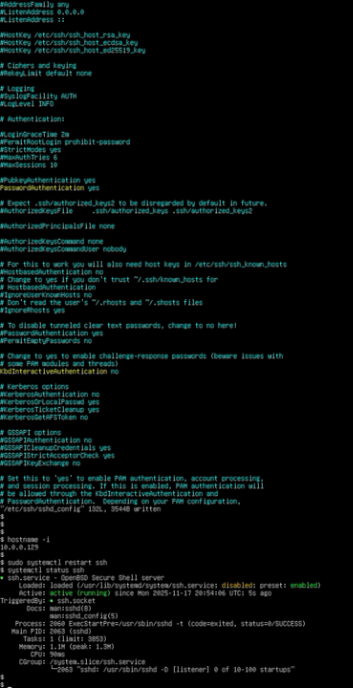
\includegraphics[width=0.5\linewidth]{Install_Images/os-firewall-ssh-config.png}
    \caption{First boot, followed by me setting up the OpenSSH server by changing the authentication config using VIM. As I didn't configure the IP config, the Pi has been assigned 10.0.0.125 via DHCP, ready for remote access}
    \label{fig:firewall-ssh}
\end{figure}

Figure \ref{fig:firewall-ssh} confirms:
\begin{itemize}
    \item The SSH service is active and running
    \item IPv4 address \texttt{10.0.0.125} assigned to \texttt{eth0} (onboard Ethernet interface)
    \item System fully accessible via SSH so screenshots can be take via a laptop and not a capture card
\end{itemize}

The base install of Ubuntu 24.04 (and other Ubuntu images) has a preconfigured Ubuntu user that, when you log in for the first time, the system asks you to change the password. If I had added my user in the additional settings page, this would not have been a problem. So when I logged in (Figure \ref{fig:firewall-load}) I changed the default user password. This practice shows Ubuntu's default security policy as it requires administrator-defined credentials instead of Ubuntu/Ubuntu.

\begin{figure}[H]
    \centering
    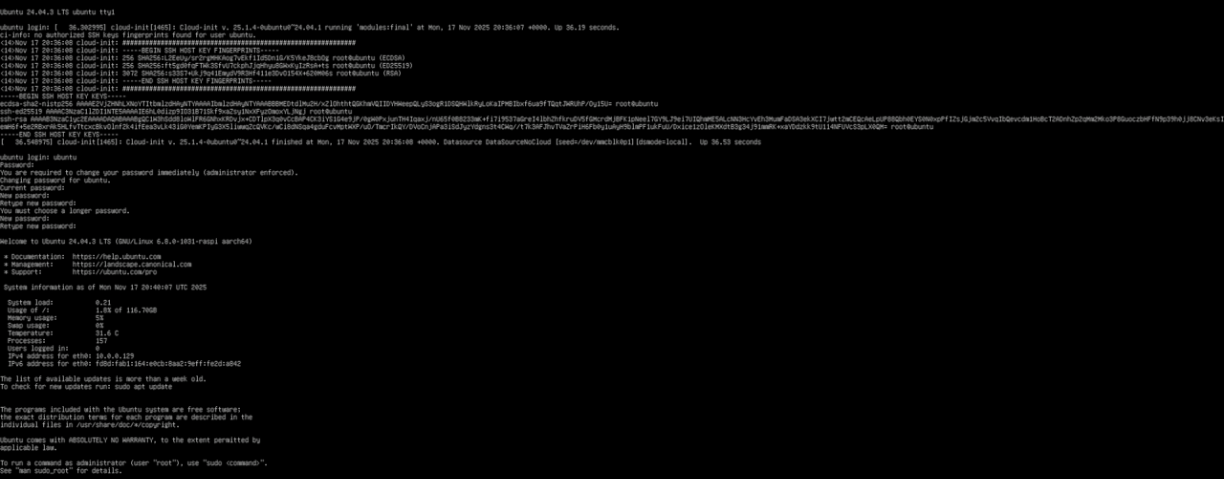
\includegraphics[width=0.95\linewidth]{Install_Images/os-firewall-load.png}
    \caption{Initial login showing mandatory password change prompt, system information (Ubuntu 24.04.3 LTS, Linux kernel 6.8.0-1051-raspi, 116.7MB memory usage), and available system updates notification.}
    \label{fig:firewall-load}
\end{figure}

Following the password change, I created my user (\texttt{s4228665}) and added myself to the sudoers file as I'll use this user to do ansible config deployments (figure \ref{fig:firewall-adduser}).

\begin{figure}[H]
    \centering
    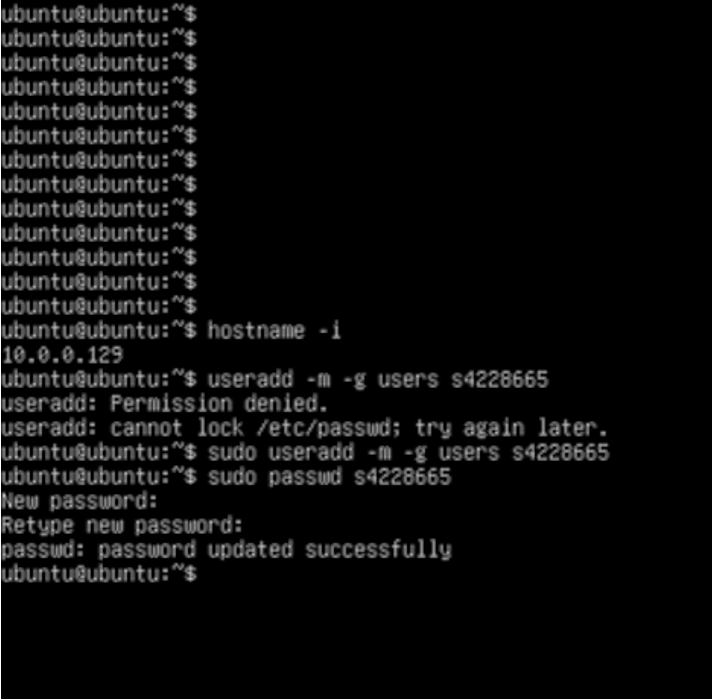
\includegraphics[width=0.95\linewidth]{Install_Images/os-firewall-add-user.png}
    \caption{Adding my user with \texttt{useradd} to create the (s4228665) user}
    \label{fig:firewall-adduser}
\end{figure}

In attempting to capture this process end-to-end elements were missed, the final step of getting my user configured and the OpenSSH server working took several tries until I was able to SSH from my laptop the first time (figure \ref{fig:firewall-first-ssh}), the main difference is when it finally worked DHCP from my local network assigned the Pi a final IP address of \verb|10.0.0.184|

\begin{figure}[H]
    \centering
    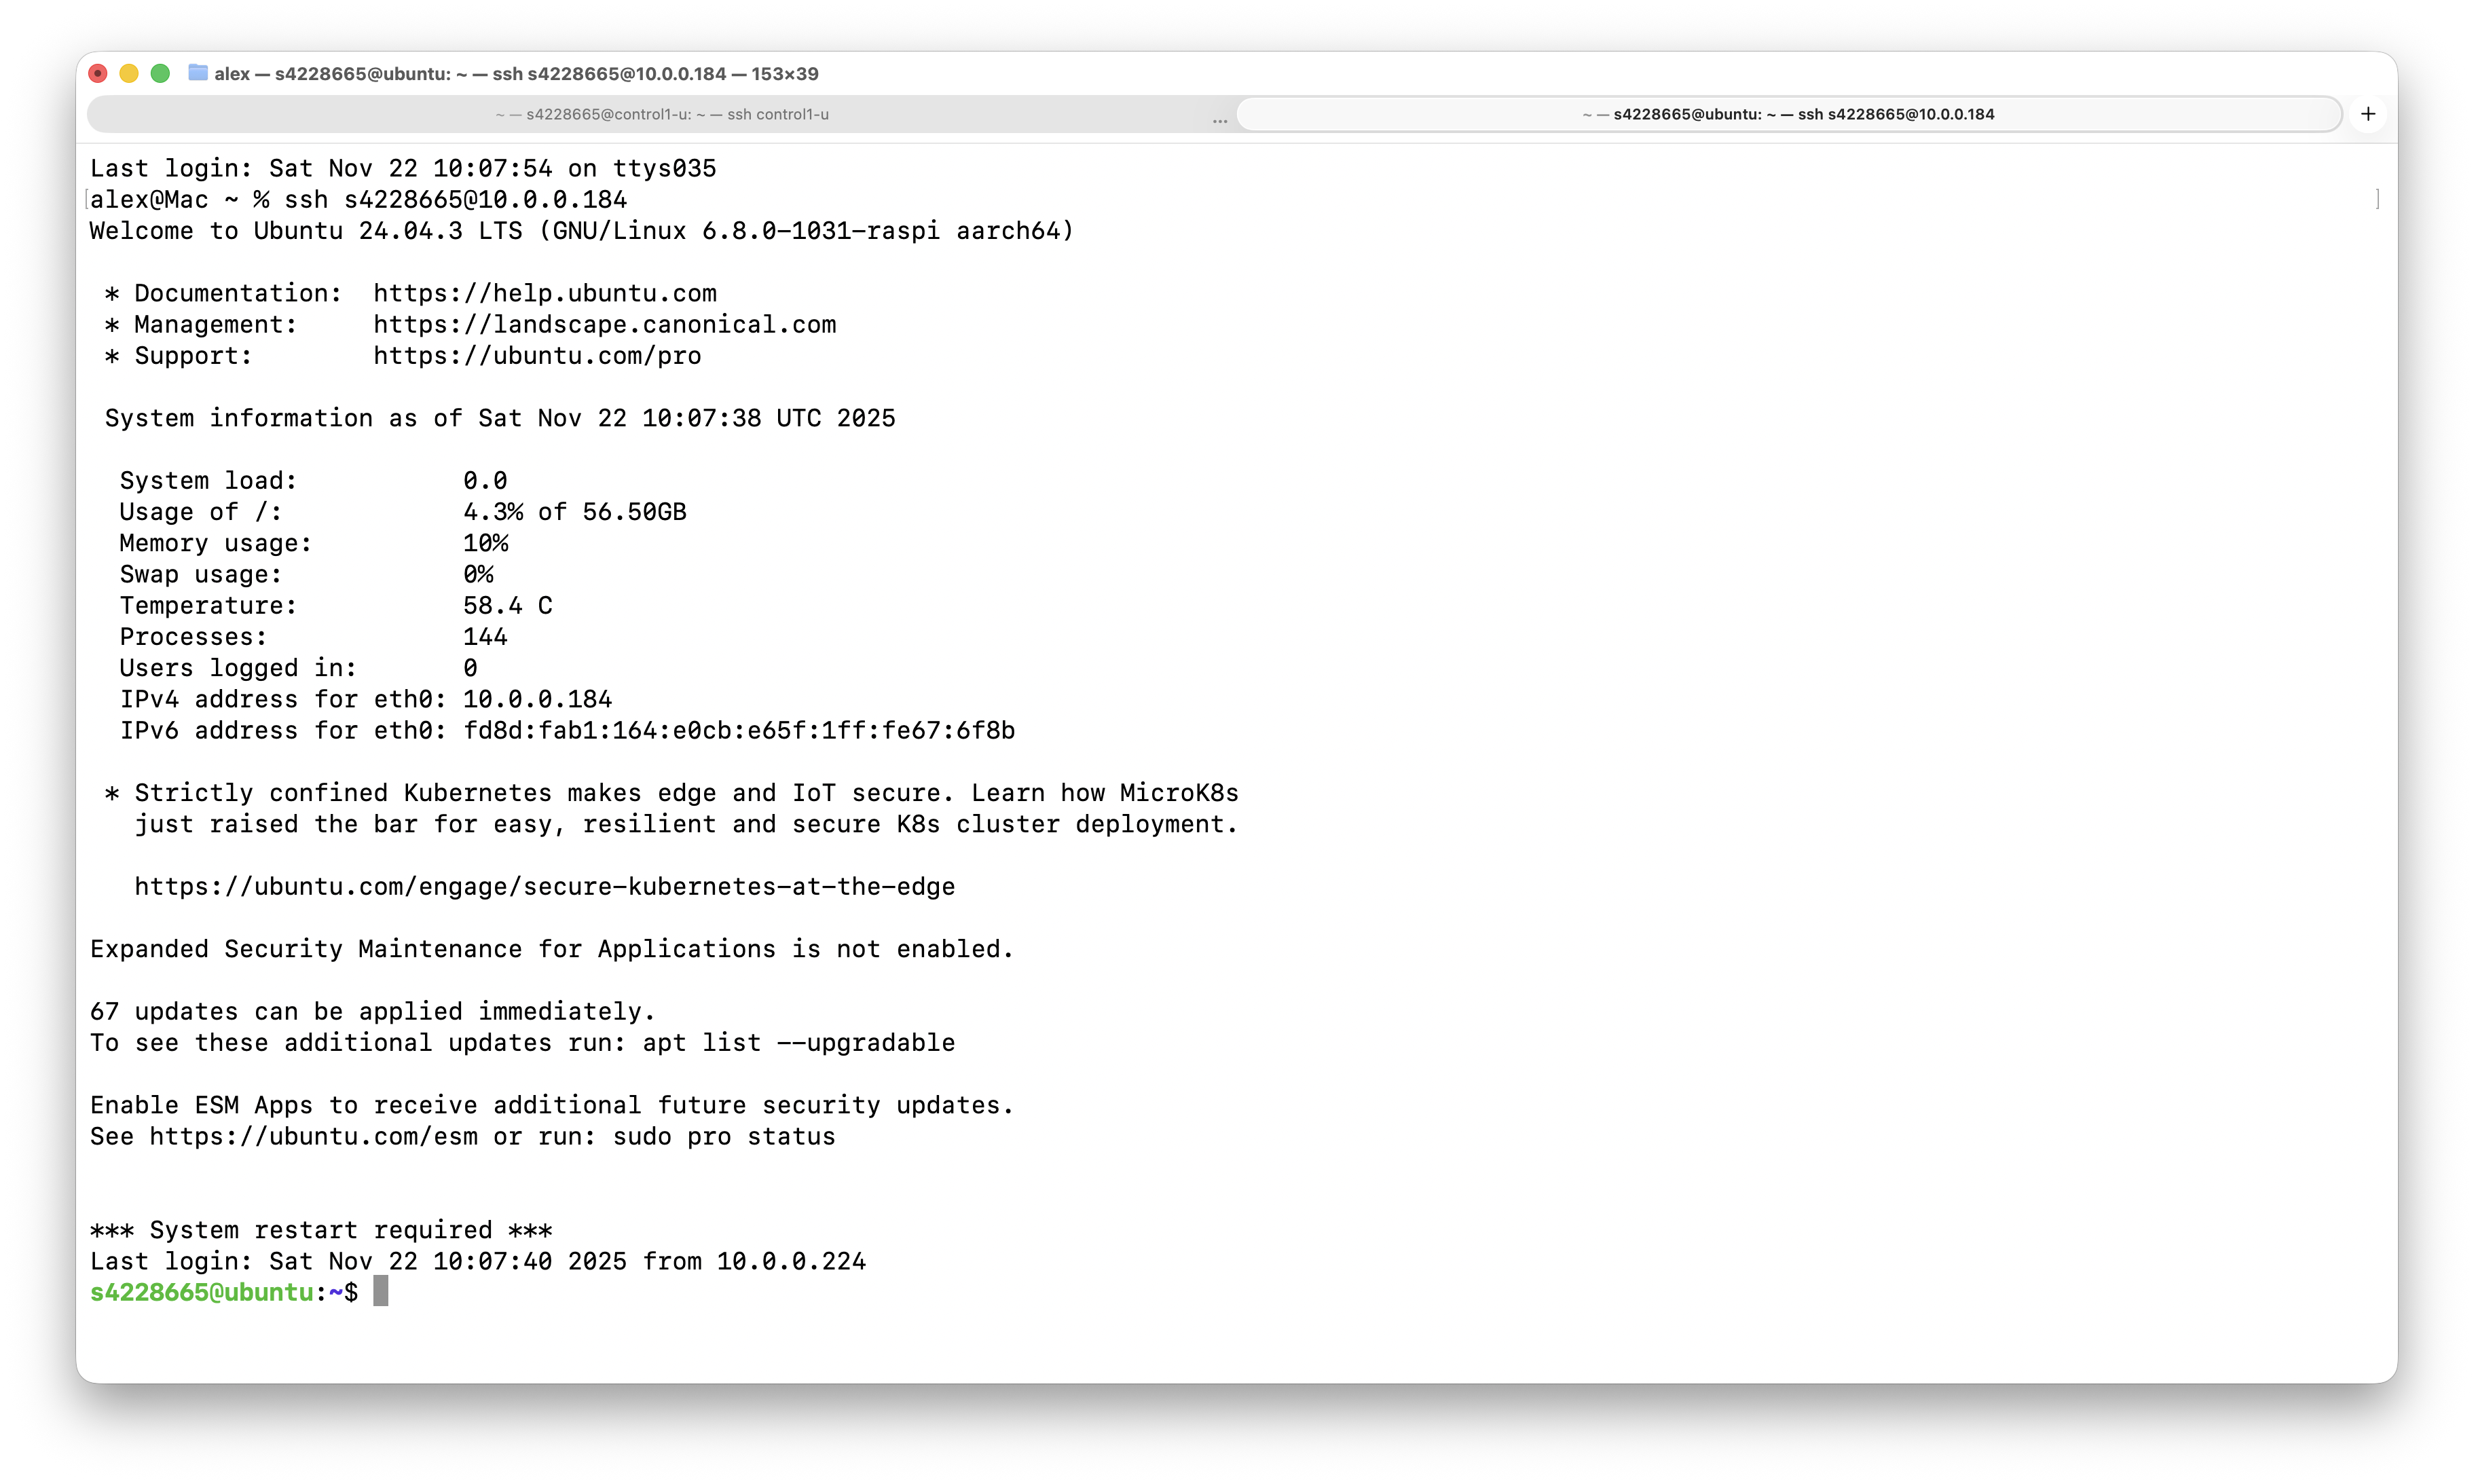
\includegraphics[width=0.95\linewidth]{Install_Images/os-alex-first-ssh.png}
    \caption{A successfull first SSH from my laptop}
    \label{fig:firewall-first-ssh}
\end{figure}